\documentclass[a4paper,11pt]{exam}
%\printanswers % pour imprimer les réponses (corrigé)
\noprintanswers % Pour ne pas imprimer les réponses (énoncé)
\addpoints % Pour compter les points
% \noaddpoints % pour ne pas compter les points
%\qformat{\textbf{\thequestion ) } }
%\qformat{\textbf{\thequestion )}} % Pour définir le style des questions (facultatif)
\usepackage{color} % définit une nouvelle couleur
\shadedsolutions % définit le style des réponses
% \framedsolutions % définit le style des réponses
\definecolor{SolutionColor}{rgb}{0.8,0.9,1} % bleu ciel
\renewcommand{\solutiontitle}{\noindent\textbf{Solution:}\par\noindent} % Définit le titre des solutions
\usepackage{gensymb}



\makeatletter

\def\maketitle{{\centering%
	\par{\huge\textbf{\@title}}%
	\par{\@date}%
	\par}}


\renewcommand{\thesubsection}{\Alph{subsection}.}   

\makeatother

\lhead{NOM Pr\'enom :}
\rhead{\textbf{Les r\'eponses doivent \^etre justifi\'ees et r\'edig\'ees}}
\cfoot{\thepage / \pageref{LastPage}}


%\usepackage{../../pas-math}
%\usepackage{../../moncours}


%\usepackage{pas-cours}
%-------------------------------------------------------------------------------
%          -Packages nécessaires pour écrire en Français et en UTF8-
%-------------------------------------------------------------------------------
\usepackage[utf8]{inputenc}
\usepackage[frenchb]{babel}
%\usepackage{numprint}
\usepackage[T1]{fontenc}
%\usepackage{lmodern}
\usepackage{textcomp}
\usepackage[french, boxed]{algorithm2e}
\usepackage{hyperref}


%-------------------------------------------------------------------------------

%-------------------------------------------------------------------------------
%                          -Outils de mise en forme-
%-------------------------------------------------------------------------------
\usepackage{hyperref}
\hypersetup{pdfstartview=XYZ}
%\usepackage{enumerate}
\usepackage{graphicx}
\usepackage{multicol}
\usepackage{tabularx}
\usepackage{multirow}
\usepackage{color}
\usepackage{eurosym}


\usepackage{anysize} %%pour pouvoir mettre les marges qu'on veut
%\marginsize{2.5cm}{2.5cm}{2.5cm}{2.5cm}

\usepackage{indentfirst} %%pour que les premier paragraphes soient aussi indentés
\usepackage{verbatim}
\usepackage{enumitem}
\usepackage{booktabs}
\usepackage[usenames,dvipsnames,svgnames,table]{xcolor}

\usepackage{variations}

%-------------------------------------------------------------------------------


%-------------------------------------------------------------------------------
%                  -Nécessaires pour écrire des mathématiques-
%-------------------------------------------------------------------------------
\usepackage{amsfonts}
\usepackage{amssymb}
\usepackage{amsmath}
\usepackage{amsthm}
\usepackage{tikz}
\usepackage{xlop}
\usepackage[output-decimal-marker={,}]{siunitx}
%-------------------------------------------------------------------------------

%-------------------------------------------------------------------------------
%                  -Nécessaires pour écrire des formules chimiquess-
%-------------------------------------------------------------------------------

\usepackage[version=4]{mhchem}

%-------------------------------------------------------------------------------
% Pour pouvoir exploiter les fichiers directement dans beamer
\newcommand{\pause}{\ }
%-------------------------------------------------------------------------------
%                    - Mise en forme avancée
%-------------------------------------------------------------------------------

\usepackage{ifthen}
\usepackage{ifmtarg}


\newcommand{\ifTrue}[2]{\ifthenelse{\equal{#1}{true}}{#2}{$\qquad \qquad$}}

%\newcommand{\kword}[1]{\textcolor{red}{\underline{#1}}}
%-------------------------------------------------------------------------------

%-------------------------------------------------------------------------------
%                     -Mise en forme d'exercices-
%-------------------------------------------------------------------------------
%\newtheoremstyle{exostyle}
%{\topsep}% espace avant
%{\topsep}% espace apres
%{}% Police utilisee par le style de thm
%{}% Indentation (vide = aucune, \parindent = indentation paragraphe)
%{\bfseries}% Police du titre de thm
%{.}% Signe de ponctuation apres le titre du thm
%{ }% Espace apres le titre du thm (\newline = linebreak)
%{\thmname{#1}\thmnumber{ #2}\thmnote{. \normalfont{\textit{#3}}}}% composants du titre du thm : \thmname = nom du thm, \thmnumber = numéro du thm, \thmnote = sous-titre du thm

%\theoremstyle{exostyle}
%\newtheorem{exercice}{Exercice}
%
%\newenvironment{questions}{
%\begin{enumerate}[\hspace{12pt}\bfseries\itshape a.]}{\end{enumerate}
%} %mettre un 1 à la place du a si on veut des numéros au lieu de lettres pour les questions 
%-------------------------------------------------------------------------------

%-------------------------------------------------------------------------------
%                    - Mise en forme de tableaux -
%-------------------------------------------------------------------------------

\renewcommand{\arraystretch}{1.7}

\setlength{\tabcolsep}{1.2cm}

%-------------------------------------------------------------------------------



%-------------------------------------------------------------------------------
%                    - Racourcis d'écriture -
%-------------------------------------------------------------------------------
%Droites
\newcommand{\dte}[1]{$(#1)$}
\newcommand{\fig}[1]{figure $#1$}
\newcommand{\sym}{symétrique}
\newcommand{\syms}{symétriques}
\newcommand{\asym}{axe de symétrie}
\newcommand{\asyms}{axes de symétrie}
\newcommand{\seg}[1]{$[#1]$}
\newcommand{\monAngle}[1]{$\widehat{#1}$}
\newcommand{\bissec}{bissectrice}
\newcommand{\mediat}{médiatrice}
\newcommand{\ddte}[1]{$[#1)$}


% Angles orientés (couples de vecteurs)
\newcommand{\aopp}[2]{(\vec{#1}, \vec{#2})} %Les deuc vecteurs sont positifs
\newcommand{\aopn}[2]{(\vec{#1}, -\vec{#2})} %Le second vecteur est négatif
\newcommand{\aonp}[2]{(-\vec{#1}, \vec{#2})} %Le premier vecteur est négatif
\newcommand{\aonn}[2]{(-\vec{#1}, -\vec{#2})} %Les deux vecteurs sont négatifs

%Ensembles mathématiques
\newcommand{\naturels}{\mathbb{N}} %Nombres naturels
\newcommand{\relatifs}{\mathbb{Z}} %Nombres relatifs
\newcommand{\rationnels}{\mathbb{Q}} %Nombres rationnels
\newcommand{\reels}{\mathbb{R}} %Nombres réels
\newcommand{\complexes}{\mathbb{C}} %Nombres complexes


%Intégration des parenthèses aux cosinus
\newcommand{\cosP}[1]{\cos\left(#1\right)}
\newcommand{\sinP}[1]{\sin\left(#1\right)}


%Probas stats
\newcommand{\stat}{statistique}
\newcommand{\stats}{statistiques}


\newcommand{\homo}{homothétie}
\newcommand{\homos}{homothéties}


\newcommand{\mycoord}[3]{(\textcolor{red}{\num{#1}} ; \textcolor{Green}{\num{#2}} ; \textcolor{blue}{\num{#3}})}
%-------------------------------------------------------------------------------

%-------------------------------------------------------------------------------
%                    - Mise en page -
%-------------------------------------------------------------------------------

\newcommand{\twoCol}[1]{\begin{multicols}{2}#1\end{multicols}}


\setenumerate[1]{font=\bfseries,label=\textit{\alph*})}
\setenumerate[2]{font=\bfseries,label=\arabic*)}


%-------------------------------------------------------------------------------
%                    - Elements cours -
%-------------------------------------------------------------------------------

%Correction d'exercice
\newcommand{\exoSec}[2]{\subsection*{Exercice #1 page #2}}
%-------------------------------------------------------------------------------
%                    - raccourcis d'écriture -
%-------------------------------------------------------------------------------

%Mise en évidence de termes clés
\newcommand{\mykw}[1]{\textcolor{red}{\underline{\textbf{#1}}}}

%Exercices
\newcommand{\exo}[2]{exercice #1 page #2}
\newcommand{\Exo}[2]{Exercice #1 page #2}

\renewcommand{\pause}{\ }

%Intervalles
\newcommand{\interOO}[2]{$]$#1 , #2$[$}
\newcommand{\interOF}[2]{$]$#1 , #2$]$}
\newcommand{\interFO}[2]{$[$#1 , #2$[$}
\newcommand{\interFF}[2]{$[$#1 , #2$]$}



%\usepackage{fullpage}
\author{\ }
\date{4 Décembre 2018}
\title{Sciences Physiques : DS n° 3}


\begin{document}
%	\usepackage{fancyhdr}
%	
%	\pagestyle{fancy}
%	\fancyhf{}
	%\rhead{Share\LaTeX}

	\maketitle
	
\begin{small}
	\begin{center}
		\begin{tabular}{|@{\ }l@{}|@{\ }c@{\ }|}
			\hline
			\textbf{Compétence} & \textbf{Maitrise} \\
			\hline
			Changements d’états de la matière \ &  \ \ \ \\
			\hline
			Conservation de la masse, variation du volume, température de changement d’état \ &  \ \ \ \\
			\hline
		\end{tabular}
	\end{center}
\end{small}	
	
	
%\vspace*{-0.5cm}	

%\section{\'Equations de réaction}

Ajuster les équations de réactions suivantes :
\begin{questions}
	\question $CH_4 + ....O_2 \rightarrow ....CO_2 + ....H_2O$
	
	\question $C_7H_{16} + ....O_2 \rightarrow ....CO_2 + ....H_2O$	
	
	\question $C_6H_{2}O + ....O_2 \rightarrow ....CO_2 + ....H_2O$
\end{questions}


%\section{À chaque modèle sa formule}
\begin{questions}
	\question \'A partir de ces dessins de modèles, donner la formule des molécules suivantes.

	\begin{center}
		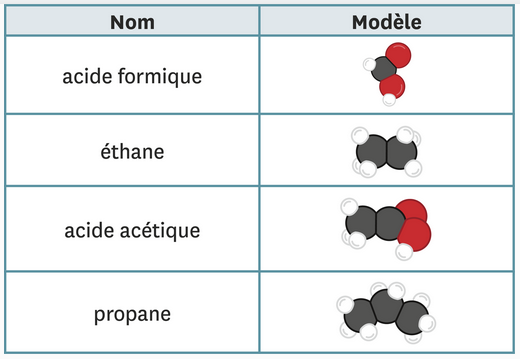
\includegraphics[scale=0.6]{img/exemples}
	\end{center}
	\fillwithdottedlines{2cm}
	
\end{questions}

%Seul l'\ref{ex:surface} est à faire sur le sujet.
Le soin et la qualité de rédaction sont pris en compte dans la notation.


%\section{Quels atomes dans cette particule ? (4 points)}\label{ex:particule}



\begin{questions}
	\question[4] Pour chaque espèce chimique, indiquer le type d'atome, le nombre d'atomes de chaque type et le nombre total d'atomes qu'elle contient.
	 
	\begin{multicols}{4}
		\begin{itemize}
			\item $CO_2$
			\item $H_2$
			\item $CH_4$
			\item $O_2$
			\item $C_4H_{10} $
			\item $C_6H_{12} O_6$
			\item $C$
			\item $H_2O$
		\end{itemize}
	\end{multicols}

	\begin{solution}
		\begin{tabular}{|@{\ }c@{\ }|@{\ }c@{\ }|@{\ }c@{\ }|@{\ }c@{\ }|@{\ }c@{\ }|}
			\hline
			Molécule         & Nombre d'atomes & Nombre d'atomes & Nombre d'atomes & Nombre total \\ 
			& de carbone      & d'hydrogène     & d'oxygène       & d'atomes         \\ \hline
			$CO_2$           & 1               & 0               & 2               & 3               \\ \hline
			$H_2$            & 0               & 2               & 0               & 2               \\ \hline
			$CH_4$           & 1               & 4               & 0               & 5               \\ \hline
			$O_2$            & 0               & 0               & 2               & 2               \\ \hline
			$C_4H_{10}$      & 4               & 10              & 0               & 14              \\ \hline
			$C_6H_{12}O_{6}$ & 6               & 12              & 6               & 24              \\ \hline
			$C$              & 1               & 0               & 0               & 1               \\ \hline
			$H_2O$           & 0               & 2               & 1               & 3               \\ \hline
		\end{tabular}
	\end{solution}
	
\end{questions}

%\newpage

\section{Une bouteille d'eau au congélateur (2 points)}\label{ex:congel}

Palmyre verse 1 L d'eau, de masse 1 kg, dans une bouteille qu'elle place ensuite au congélateur. Après quelques heures, la bouteille est déformée.

\begin{questions}
	\question[1] Que vaut alors la masse de l'eau contenue dans la bouteille ?
	\begin{solution}
		La masse d'un corps ne change pas lors du changement d'état, donc la masse de l'eau contenue dans la bouteille est toujours 1 kg.
	\end{solution}
	
	\question[1] Que peut-on dire du volume d'eau contenu dans la bouteille ?
	\begin{solution}
		Lors de la solidification, le volume augmente donc le volume de l'eau a augmenté.
	\end{solution}
\end{questions}


%\section{La phrase mystère (2 points)}

Construire une phrase expliquant ce qui se passe dans le compartiment à glace d'un réfrigérateur lorsqu'on fabrique des glaçons, en utilisant les expressions suivantes :

\begin{multicols}{3}
	\begin{itemize}
		\item se solidifie
		\item cède de l'énergie
		\item l'eau liquide
		\item à l'air
		\item température de 0°C
	\end{itemize}
\end{multicols}

%\section{Brouillard : gaz ou liquide ?}

Alexandre fait chauffer de l'eau pour faire cuire des pâtes. Quand l'eau arrive à ébullition, il passe rapidement sa main dans le <<brouillard>> au-dessus de la casserole.

Expliquer pourquoi la main d'Alexandre est alors humide ?

\section{Chauffer de l'eau pour faire cuire du riz (4 points)}

Pour la cuisson du riz, on peut lire sur le paquet : << verser un volume de riz dans 5 volumes d'eau bouillante >>.

\begin{questions}
	\question[1\half] Indiquer ce que fournit le dispositif de chauffage pour augmenter la température de l'eau.
	
	\question[1\half] Pourquoi il faut fournir plus d'énergie lorsque l'on met initialement dans la casserole de l'eau froide, plutôt que de l'eau chaude, pour la porter à ébullition ?
	
	\question[1] Indiquer à quoi sert l'énergie fournie par la plaque électrique, une fois l'eau à ébullition.
\end{questions}

\section{Réaliser des soudures sur les circuits (3 points)}

En électronique, pour fixer un composant sur un circuit imprimé, on fait fondre un fil d'étain (métal dont la température de fusion est 232 °C) avec un fer à souder. La goutte d'étain déposée sur le circuit refroidit, fixant ainsi le composant sur le circuit.

\begin{questions}
	\question[1] Donner le nom du changement d'état subit par l'étain lorsqu'on le chauffe au fer à souder.
	
	\question[1] Nommer le changement d'état subit par la goutte d'étain sur le circuit en refroidissant.
	
	\question[1] Justifier l'utilisation de l'étain pour effectuer les soudures plutôt que le fer dont la température de fusion est de \num{1535} °C.  
\end{questions}

\newpage

\section{La température qui monte (4 points)}\label{ex:fusion}

Dans un récipient qui contient de l'eau, on a placé un thermomètre. On l'a placé au congélateur pendant une nuit avant de le sortir. On a relevé la température de l'eau toutes les 10 min.

\begin{center}
	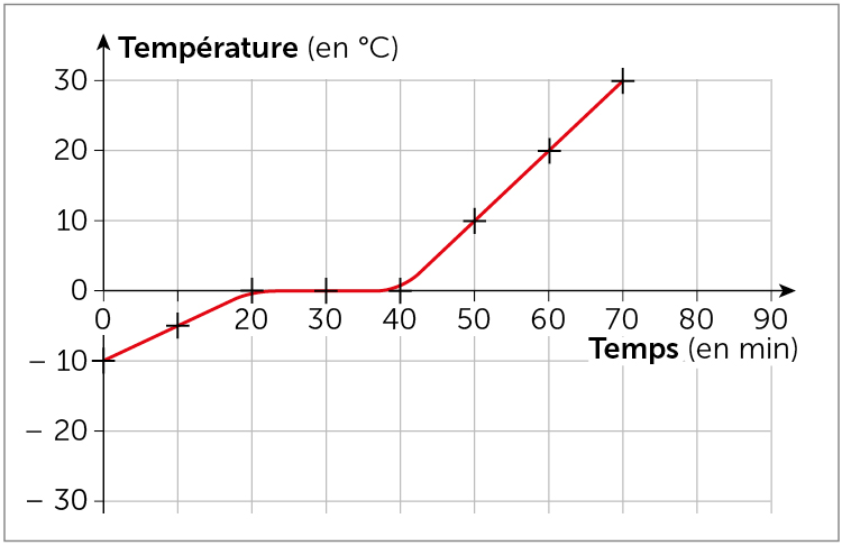
\includegraphics[scale=0.4]{./img/courbe}
\end{center}

\begin{questions}
	\question[2] Quel est l'état de l'eau après 10 minutes ? Après 60 minutes ?
	\begin{solution}
		Après 10 min, la température est inférieure à 0°C donc l'eau est solide. Après 60 min, le température est supérieure à 0°C, donc l'eau est liquide.
	\end{solution}
	
	\question[1] Combien de temps a duré le changement d'état ?
	\begin{solution}
		Sur la courbe, il y a un palier de température à 0°C entre 20 et 40 min, donc le changement d'état a duré 20 min.
	\end{solution}
	
	\question[1] A quel instant n'y a-t-il plus d'eau solide dans le récipient. 
	\begin{solution}
		Il n'y a aura plus d'eau solide dans le récipient à la fin du changement d'état, donc à 40 min.
	\end{solution}
\end{questions}
 


\section{Mais quelle est donc cette matière ? (4 points)}

Nolan ne se rappelle plus quel plastique il doit acheter pour son imprimante 3D : de l'ABS ou du PLA ?

\begin{itemize}
	\item \textbf{L'ABS} est un plastique courant, on le retrouve dans les Lego par exemple. Son point fort vient de sa solidité, il commence à fondre à 180°C.
	
	\item Issu de matériaux recyclés, tels que l'amidon de maïs \textbf{le PLA} est une matière plus naturelle et biodégradable. Sa température de fusion est de 160°C.	
\end{itemize}

\begin{questions}
	\question[2] Quelle expérience Nolan peut-il réaliser pour identifier le plastique de son imprimante ?
		\begin{solution}
			Pour identifier le plastique utilisé par son imprimante, Nolan doit déterminer sa température de fusion. Pour cela il va faire chauffer le plastique jusqu'à le faire fondre en relevant régulièrement la température.
		\end{solution}
	
	\question[2] Il trace l'évolution de la température pendant la fusion du plastique. Quel est le plastique de son imprimante ?
		\begin{center}
			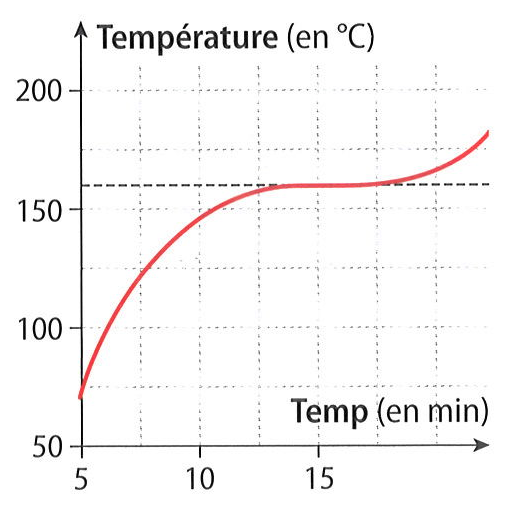
\includegraphics[scale=0.45]{./img/courbe2}
		\end{center}

		\begin{solution}
			Sur le graphique, le palier se situe entre 150°C et 175°C, ce ne peut pas être de l'ABS qui fond à une température plus importante (180°C). C'est donc du PLA qui fond à 162°C.
		\end{solution}	

\end{questions}


\ \label{LastPage}

\end{document}